\documentclass[conference]{IEEEtran}
\IEEEoverridecommandlockouts
% Package configuration for standard IEEE formatting and clean rendering
\usepackage{cite}
\usepackage{amsmath,amssymb,amsfonts}
\usepackage{algorithmic}
\usepackage{graphicx}
\usepackage{textcomp}
\usepackage{xcolor}
\usepackage{booktabs}
\usepackage{array}
\usepackage{url}
\usepackage{microtype}
\usepackage{balance}
\usepackage{tikz}
\usepackage{pgfplots}
\pgfplotsset{compat=1.18}
\usetikzlibrary{shapes,shapes.geometric,arrows,positioning,calc}

\def\BibTeX{{\rm B\kern-.05em{\sc i\kern-.025em b}\kern-.08em
    T\kern-.1667em\lower.7ex\hbox{E}\kern-.125emX}}

% Replace default em-dash in Abstract and Index Terms with clean hyphen
\makeatletter
\renewenvironment{abstract}{%
  \normalfont\footnotesize
  \bfseries\textit{Abstract} - \normalfont\footnotesize\ignorespaces
}{%
  \vspace{0.6ex}\par
}
\renewenvironment{IEEEkeywords}{%
  \normalfont\footnotesize
  \bfseries\textit{Index Terms} - \normalfont\footnotesize\ignorespaces
}{%
  \vspace{1.2ex}\par
}
\makeatother

\begin{document}

\title{SpendSense: An On-Device Multi-Task Deep Learning Framework for Privacy-Preserving Financial Telemetry and Expense Optimization in India's UPI Ecosystem}

\author{\IEEEauthorblockN{Aayush Pandey\textsuperscript{1}, Ansh Verma\textsuperscript{2}, Atharva Achare\textsuperscript{3}}
\IEEEauthorblockA{\textit{Department of Computer Science \& Engineering} \\
\textit{Bharati Vidyapeeth (Deemed to be University) Department of Engineering \& Technology}, Navi Mumbai, India \\
Email: \textsuperscript{1}aayush.pandey-detnm@bvp.edu.in, \textsuperscript{2}ansh.verma-detnm@bvp.edu.in, \textsuperscript{3}atharva.achare-detnm@bvp.edu.in}
}

\maketitle

\begin{abstract}
The rapid rise of digital payments in India has left many people juggling between UPI apps, credit cards, BNPL, and subscriptions to manage their finances. Empirical studies indicate that approximately 75\% of Indian UPI users report increased overspending attributable to the intangible nature of cashless transactions, yet no existing solution provides a unified, privacy-preserving financial dashboard tailored to India's payment ecosystem. This paper presents SpendSense, a Flutter-based mobile application that addresses this gap by automatically ingesting transaction data from bank and UPI SMS notifications on-device, without requiring account linking, password sharing, or cloud connectivity. The system employs a single multi-task TensorFlow Lite model, trained on a combined corpus of real and synthetically augmented Indian transaction data, to simultaneously predict merchant identity, spending category, subcategory, payment mode, and transaction type from raw SMS text in one forward pass. A masked multi-task loss function enables training across heterogeneous datasets where label availability varies per field. All transaction data is persisted exclusively in a local SQLite database on the user's device, ensuring zero data exposure. Additional features include proactive budget alerts at 80\% category utilization delivered via on-device notifications, automatic recurring-charge detection for forgotten subscriptions, multi-bank account aggregation, and weekly plain-English spending summaries generated from rule-based sentence templates without any external API dependency. SpendSense demonstrates that a fully offline, privacy-first personal finance system can deliver intelligent, India-specific financial insights at zero recurring infrastructure cost.
\end{abstract}

\begin{IEEEkeywords}
Personal Finance Management, UPI, Transaction Categorisation, Multi-Task Learning, On-Device Machine Learning, TensorFlow Lite, SMS Parsing, Flutter, Financial Awareness, Indian Digital Payments
\end{IEEEkeywords}

\section{Introduction}
In the last ten years the global financial environment has seen a rapid shift towards digital methods of payment. In emerging digital economies, and specifically in India, the widespread use of the UPI has created an environment in which retail micropayments take place almost instantly with very little difficulty. Statistics released by the NPCI show that the number of digital transactions has gone beyond tens of billions of monthly settlements, with physical banknotes now being replaced as the main means of daily consumer exchange.

Nevertheless, the frictionless way of settling transactions brings about serious problems relating to behaviour. In the field of classical consumer psychology, the physical resistance involved in handing over cash acts as a natural mental barrier against making impulsive purchases. On the other hand, digital micropayments separate the act of consuming from the sense of depleting one's funds. Studies in this area, for example the empirical research carried out by Dev et al. \cite{dev2024}, show that about three-quarters of the actively using digital payment users interviewed admit to making unplanned spending which can be directly linked to the intangible character of digital wallets, credit limits, and Buy Now Pay Later (BNPL) services \cite{gerrans2021}.

This psychological difficulty is worsened by the way personal finance is organised operationally. Today's retail users spread their spending across between six and eight different transaction apps, such as multi-bank portals, digital wallets, credit aggregators, and unmonitored digital subscriptions. Since each financial platform operates within its own isolated data silo, consumers do not have a clear and integrated overview of their total cash flow \cite{kaiser2022}.

Existing commercial Personal Finance Management (PFM) solutions fail to resolve this crisis due to architectural compromises \cite{pew2022}. Mainstream platforms frequently rely on cloud-centralized account scraping, demanding sensitive bank credentials, session cookies, or continuous cloud synchronization of private transaction metadata. Recent third-party PFM utilities have been shown to transmit merchant identities, balances, and geographic coordinates to remote servers, exposing consumers to severe privacy vulnerabilities. Furthermore, legacy platforms are predominantly descriptive; they summarize historical expenses at monthly billing cycles rather than offering real-time, proactive risk deterrence \cite{compen2022}.

In order to address these structural limitations, this paper introduces \textbf{SpendSense}, an entirely autonomous, offline-first personal financial analysis platform that has been implemented using Flutter. SpendSense introduces a new on-device operating framework which combines deterministic SMS parsing, local relational data storage, proactive budget exhaustion modelling, and an on-device multi-task deep neural network compiled into TensorFlow Lite. The main contributions points of this review are as follows:
\begin{enumerate}
    \item \textbf{Privacy-Preserving On-Device Ingestion:} An automated data pipeline with no use of the cloud which intercepts and interprets transactional SMS notifications locally based on recognised banking headers, thus entirely removing any exposure of third-party credentials.
    \item \textbf{Unified Multi-Task Classification Engine:} A Multi-Task Learning (MTL) architecture that is deployed on the device and is able to predict the merchant identity, the canonical expense category, the fine-grained subcategory, the transaction mechanism, and the debit/credit orientation all in one forward pass with a latency of less than one millisecond.
    \item \textbf{Masked Loss for Heterogeneous Corpora:} A masked multi-task cross-entropy loss approach which enables robust joint model convergence when training on multiple-source datasets that have incomplete label coverage.
    \item \textbf{Proactive solvency and recurrence safeguards:} an autonomous edge analysis engine which issues predictive budget warnings when 80\% of the category budget is used, detects dormant recurring subscriptions by matching temporal periodicity, and produces plain-English weekly summaries by means of deterministic natural language templates without having to rely on external large language model (LLM) API dependencies \cite{lusardi2014}.
\end{enumerate}

\section{Literature Review}
Research into automated personal finance management has been greatly stimulated by the coming together of mobile computing, consumer behavioral economics, and edge machine learning \cite{xiao2016}.

\subsection{Cashless Behavior and Expenditure Awareness}
The issue of the psychological aspect of payment settlement has for a long time been examined within the field of behavioural economics. Early research carried out by Prelec and Loewenstein showed that payment systems which separate consumption from the loss of cash greatly increase people's willingness to make purchases. In relation to India's rapid shift to UPI, Dev et al. \cite{dev2024} carried out a systematic analysis of user perceptions among different demographic groups and found that more than 75\% of the respondents noticed an increase in their spending speed after making the switch to a cashless system. Simanjuntak and Lestari \cite{simanjuntak2025} and Gerrans et al. \cite{gerrans2021} stated that although instruction in financial literacy offers basic economic knowledge, true behavioural compliance in real-life situations demands continuous and automated contextual feedback. Comp{\'e}n et al. \cite{compen2022} and Kaiser et al. \cite{kaiser2022} noted that static educational interventions do not succeed in changing habit loops unless they are supported by ongoing, actionable decision assistance.

\subsection{Expense Parsing and Financial Telemetry}
In the past, automated financial tracking has depended on Open Banking APIs or on manually keeping records in spreadsheets. In areas where there is no access to a unified API or where privacy concerns stop data from being aggregated in the cloud, SMS telemetry acts as a useful method for extracting data. The WONGA framework \cite{wonga2023} showed that it is possible to parse streams of telecommunication SMS messages in order to obtain bank balances and the amounts of purchases. Likewise, the SmartSpend paradigm \cite{smartspend2025} suggested combining spending forecasting with recommendation dashboards. Nevertheless, the current academic prototypes either require remote server telemetry, which causes a leakage of privacy, or do not provide support for region-specific syntax such as the Virtual Payment Address (VPA) strings used in India (for example, \texttt{merchant@bank}) and unstructured merchant abbreviations.

\subsection{Financial Transaction Categorization}
The task of automatically mapping raw financial strings is a particularly difficult Natural Language Processing (NLP) problem because of the severe truncation of the strings, the use of non-standard abbreviations, and the presence of numeric noise \cite{huang2021}. Toran et al. \cite{toran2023} created a weakly supervised pipeline for classifying bank transactions, using custom embeddings and Snorkel label models, for large-scale enterprise banking in the cloud. Dong et al. \cite{dong2025} introduced Txn-BERT for hierarchical classification inside accounting software. Although these cloud-based models are able to achieve good classification performance, their large number of parameters makes it impossible to run them on mobile chipsets at the edge. The LiteMuL architecture, proposed by Kumari et al. \cite{kumari2021}, showed that multi-task learning with shared encoder representations greatly reduces the size of models used for sequence tagging. SpendSense takes this edge approach further by introducing a single, compact multi-task network designed for Indian digital payments. A comparative taxonomy is given in Table~\ref{tab:comparison_apps}.

\begin{table}[htbp]
\caption{Comparison of Existing Financial Applications with SpendSense}
\label{tab:comparison_apps}
\centering
\raisebox{-30.14493pt}[32.81412pt][30.14493pt]{\makebox[254.80225pt][c]{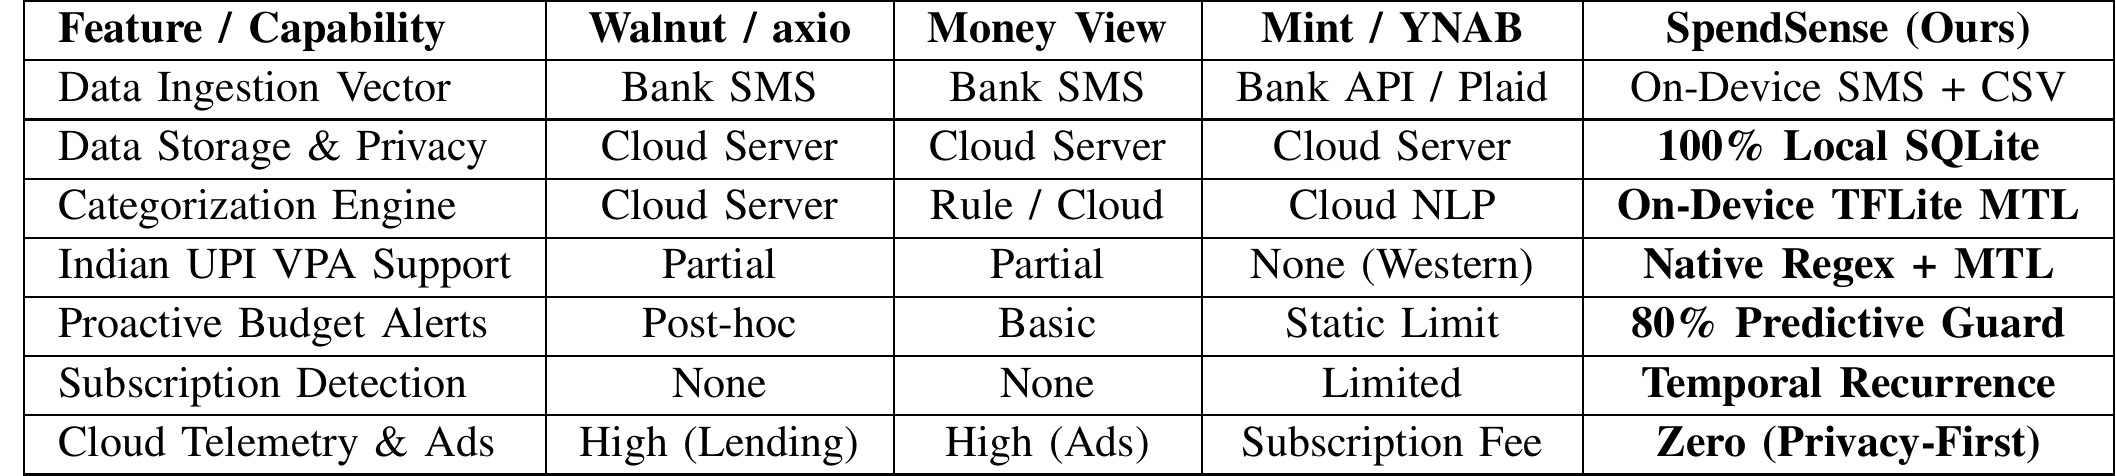
\includegraphics[width=254.80225pt,height=62.95905pt,keepaspectratio]{ieee_images/tab_comparison_apps.png}}}
\end{table}

\section{Methodology}

\subsection{Problem Definition}
Modern consumers are overwhelmed with a variety of financial utilities, from expense loggers, commercial banking software, and fragmented budgeting portals \cite{pew2022}. Users must manually toggle across applications to reconstruct their monthly cash flow, resulting in a lack of holistic financial visibility and impulsive spending behaviors.

Furthermore, most applications are purely retroactive, analyzing users balances from past months, not predicting future financial distress \cite{huang2021}.

This paper proposes \textbf{SpendSense}: an end to end framework consisting of automated transaction ingestion, overspending risk prediction, and on-device intelligent decision support.

\subsection{System Architecture}
The system is organized according to an efficient, modular, and microservices-like architecture that emphasizes high-level throughput and scalability. The application segregates its primary operations into four distinct stages:
\begin{itemize}
    \item \textbf{The client-side:} built with Flutter widgets, is responsible for visualizing the information, managing expenses, and maintaining user preferences.
    \item \textbf{API and Ingestion Tier:} The second stage operates as an API and ingestion layer, which performs the transaction parsing, regex normalization, and database updates in the local machine.
    \item \textbf{Machine Learning Inference Tier:} The third stage involves the machine learning inference layer, which is implemented as a set of high-performance microservices in the development stage and compiled into a low-sized tensorflow lite model for the production-ready application \cite{pedregosa2011}. This step executes the prediction algorithms for expenses’ categories, merchants, and potential budget risks.
    \item \textbf{Persistence Tier:} Finally, the persistence layer stores the application’s data as an encrypted local SQLite database.
\end{itemize}

\begin{figure}[htbp]
\centering
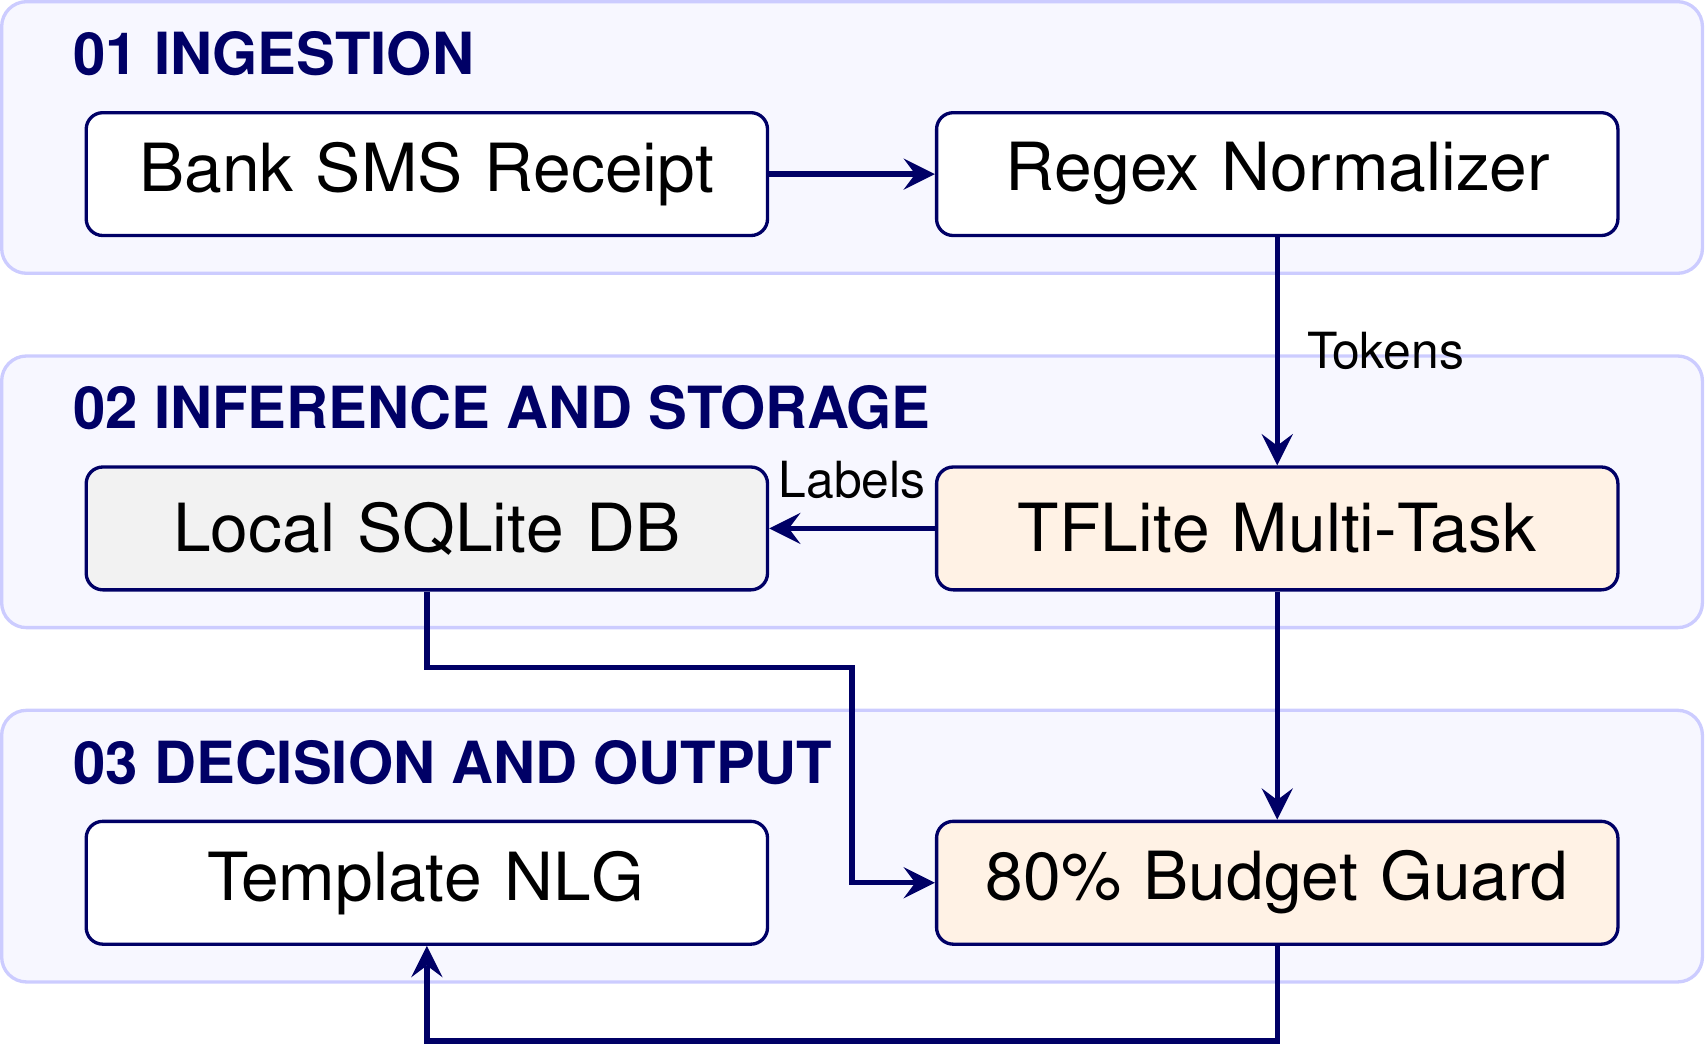
\includegraphics[width=191.08876pt,height=122.64818pt,keepaspectratio]{ieee_images/fig_pipeline_architecture.png}
\caption{End-to-end local data ingestion, multi-task classification, and proactive budget notification pipeline of the SpendSense architecture.}
\label{fig:pipeline_architecture}
\end{figure}

\subsection{Dataset Description}
The model is trained on a real-world corpus of Indian digital payments, banking SMS, and synthetically augmented records \cite{chen2016}, where raw financial strings are preprocessed into tokens, extracted virtual payment addresses (e.g., \texttt{merchant@bank}), masked sensitive personal information, and temporal features are extracted.

The corpus consists of 107,455 instances involving 734 unique merchants and 15 standard spending categories (Food, Groceries, Shopping, Entertainment, Utilities, Transport, Fuel, Housing, Medical, Education, Travel, EMI, Subscription, Income, Personal) used to train the model (see Table ~\ref{tab:dataset_desc} for details). The data is split into an 80\% training set (85,925), 10\% validation set (10,765), and 10\% test set (10,765).

\begin{table}[htbp]
\caption{SpendSense Transaction Dataset Composition and Partition}
\label{tab:dataset_desc}
\centering
\raisebox{-25.11182pt}[28.22530pt][25.11182pt]{\makebox[254.80202pt][c]{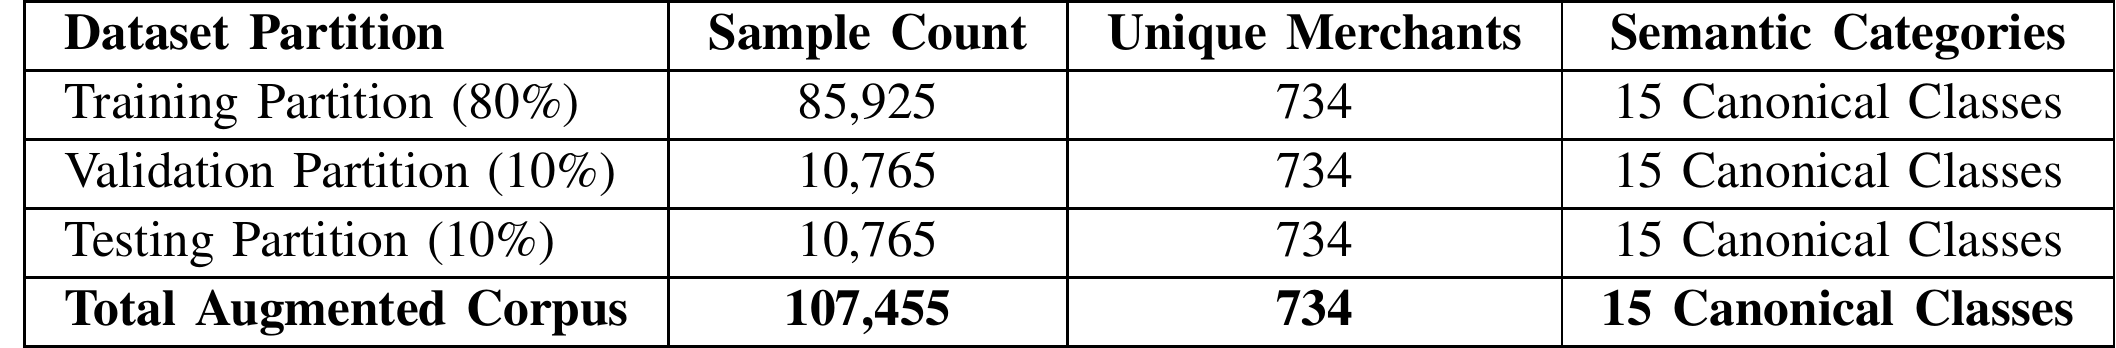
\includegraphics[width=254.80202pt,height=53.33712pt,keepaspectratio]{ieee_images/tab_dataset_desc.png}}}
\end{table}

The data was standardized to include tuples of Credit/Debit, numerical amount of the transaction, spending category, timestamp, and encrypted user tokens.

\subsection{Feature Engineering}

The raw data is then converted to densely formatted features to capture the underlying regularities in the data \cite{breiman2001}.

There are six engineered features, described in Table~\ref{tab:engineered_features}.

\begin{table}[htbp]
\caption{Engineered Behavioral Features and Domain Semantics}
\label{tab:engineered_features}
\centering
\raisebox{-34.82474pt}[38.82474pt][34.82474pt]{\makebox[271.64482pt][c]{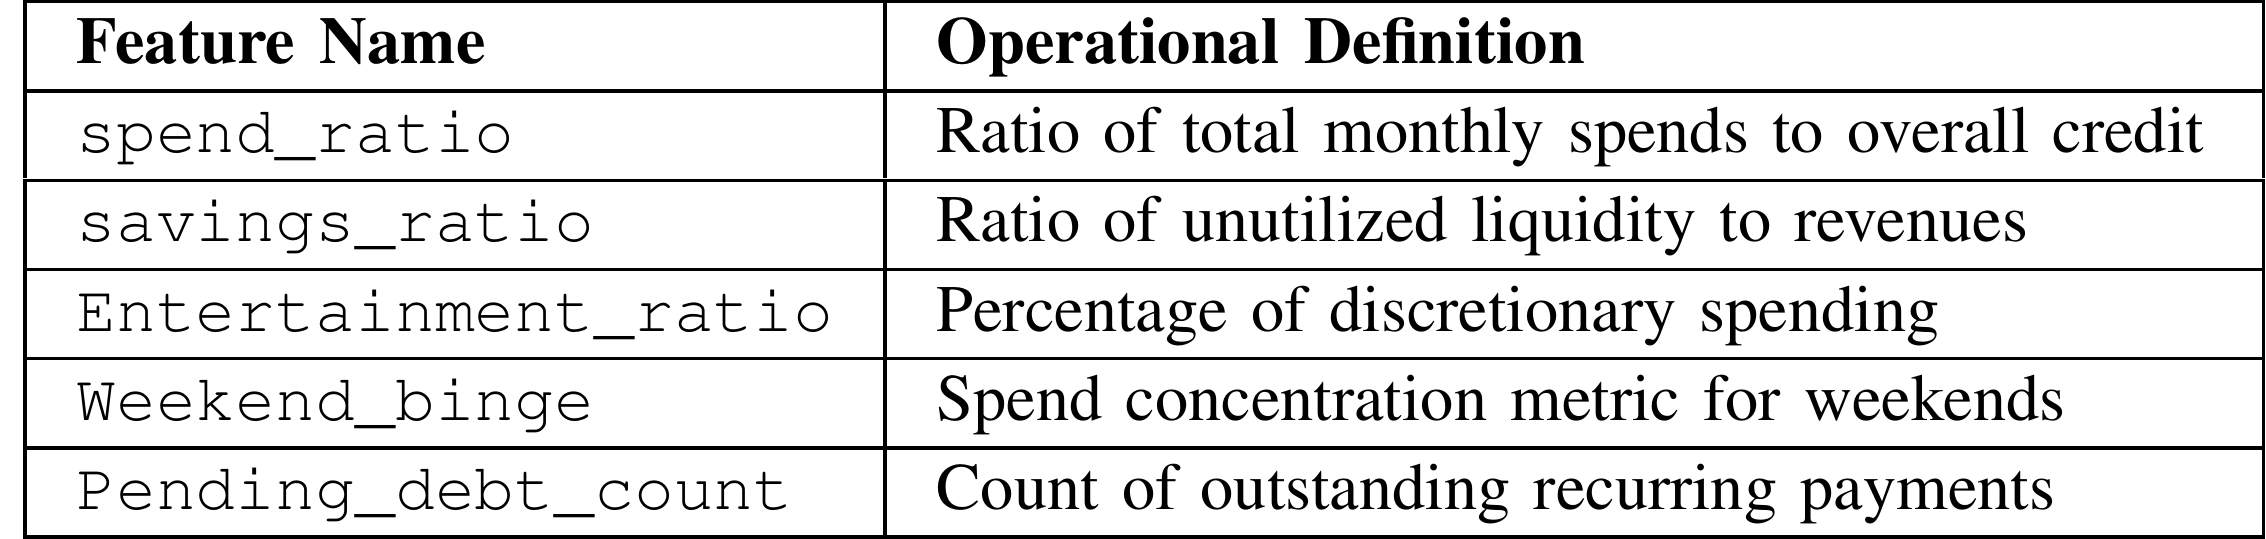
\includegraphics[width=271.64482pt,height=73.64948pt,keepaspectratio]{ieee_images/tab_engineered_features.png}}}
\end{table}

\begin{figure}[htbp]
\centering
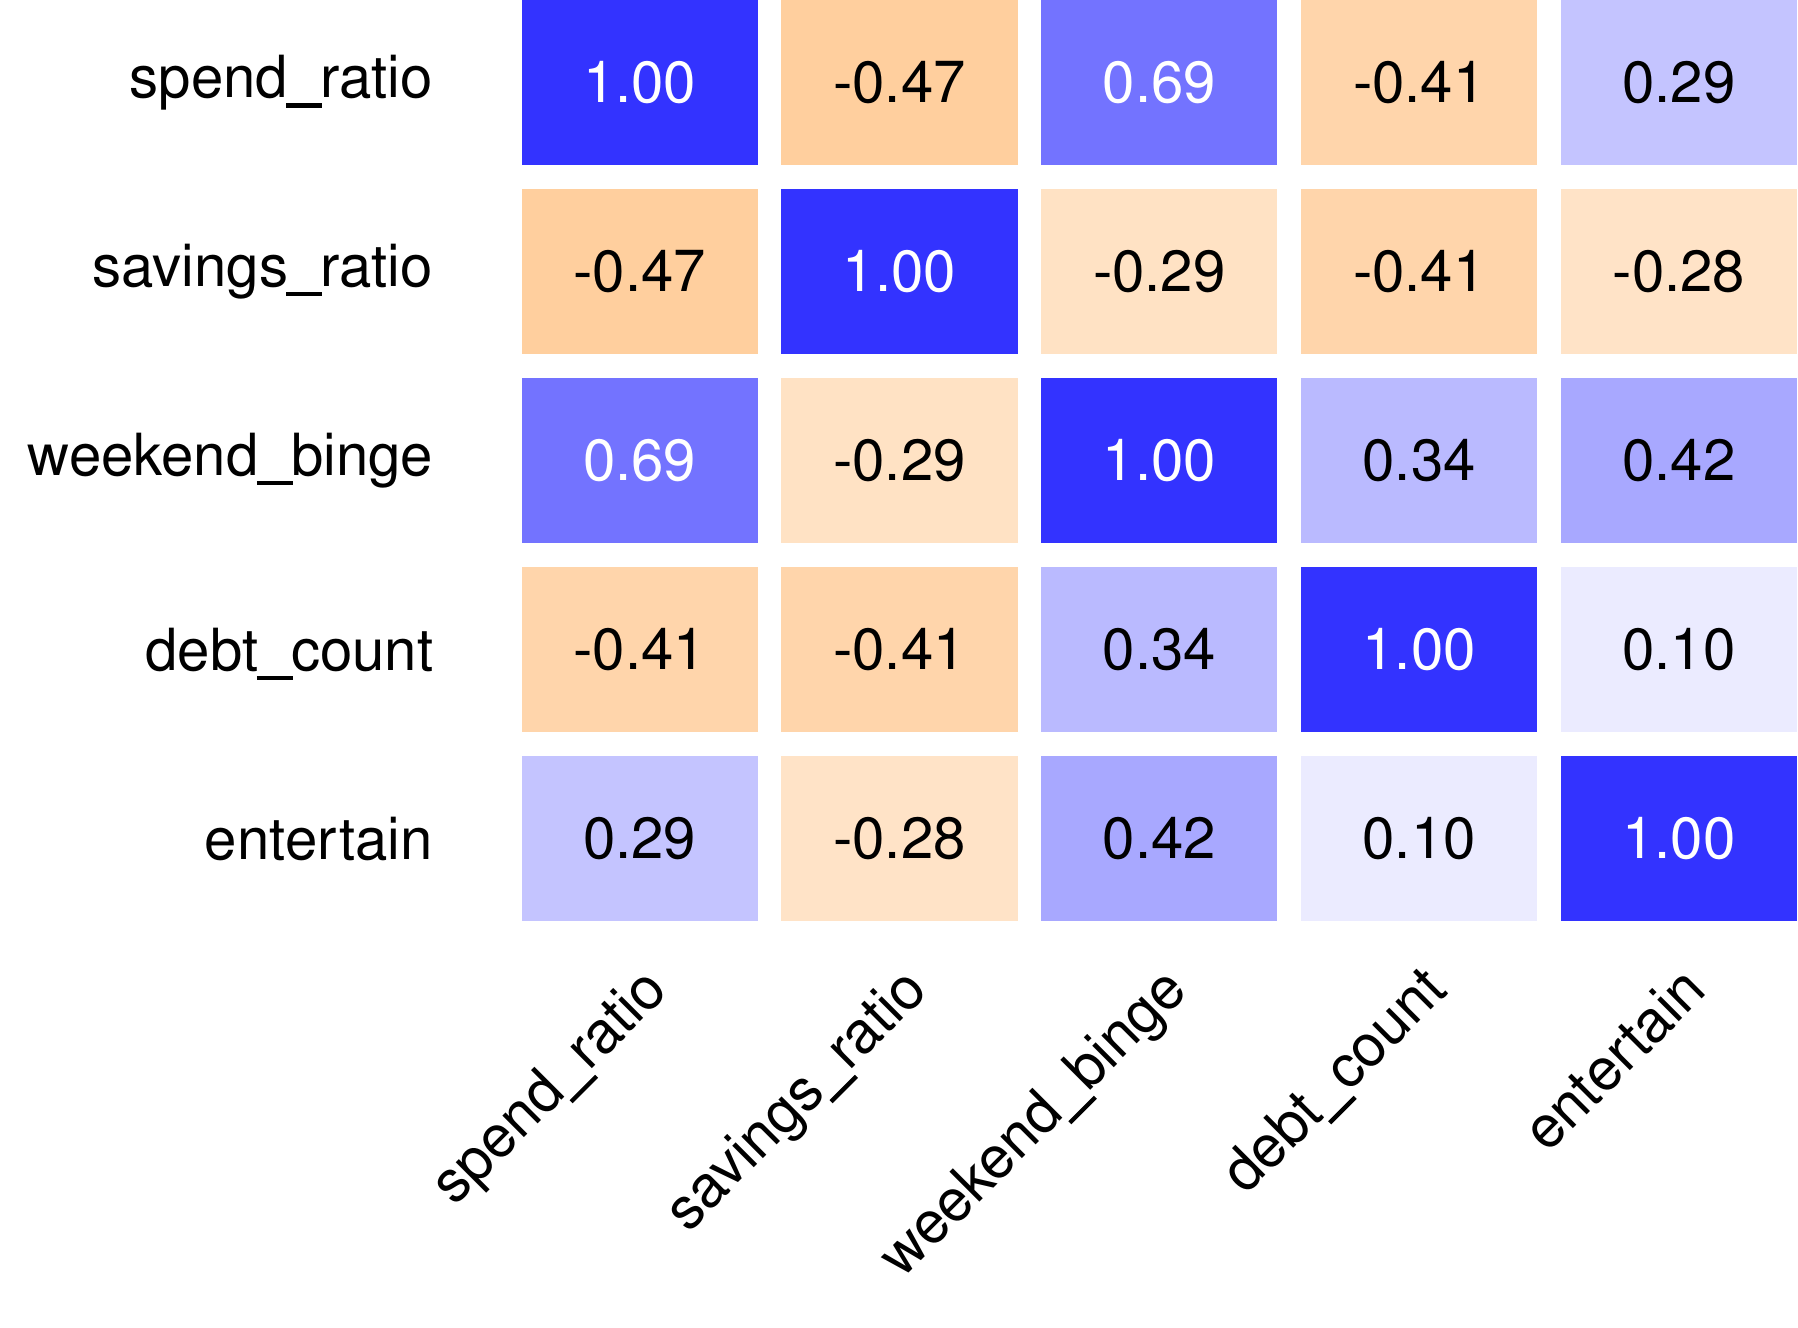
\includegraphics[width=161.96145pt,height=123.75559pt,keepaspectratio]{ieee_images/fig_correlation_matrix.png}
\caption{Correlation Matrix of Engineered Financial Features.}
\label{fig:correlation_matrix}
\end{figure}

These engineered signals capture holistic financial patterns beyond raw debit totals \cite{friedman2001}. Fig.~\ref{fig:correlation_matrix} illustrates the correlation topology, demonstrating strong interrelationships between discretionary weekend activity and overall expenditure velocity.

\begin{figure}[htbp]
\centering
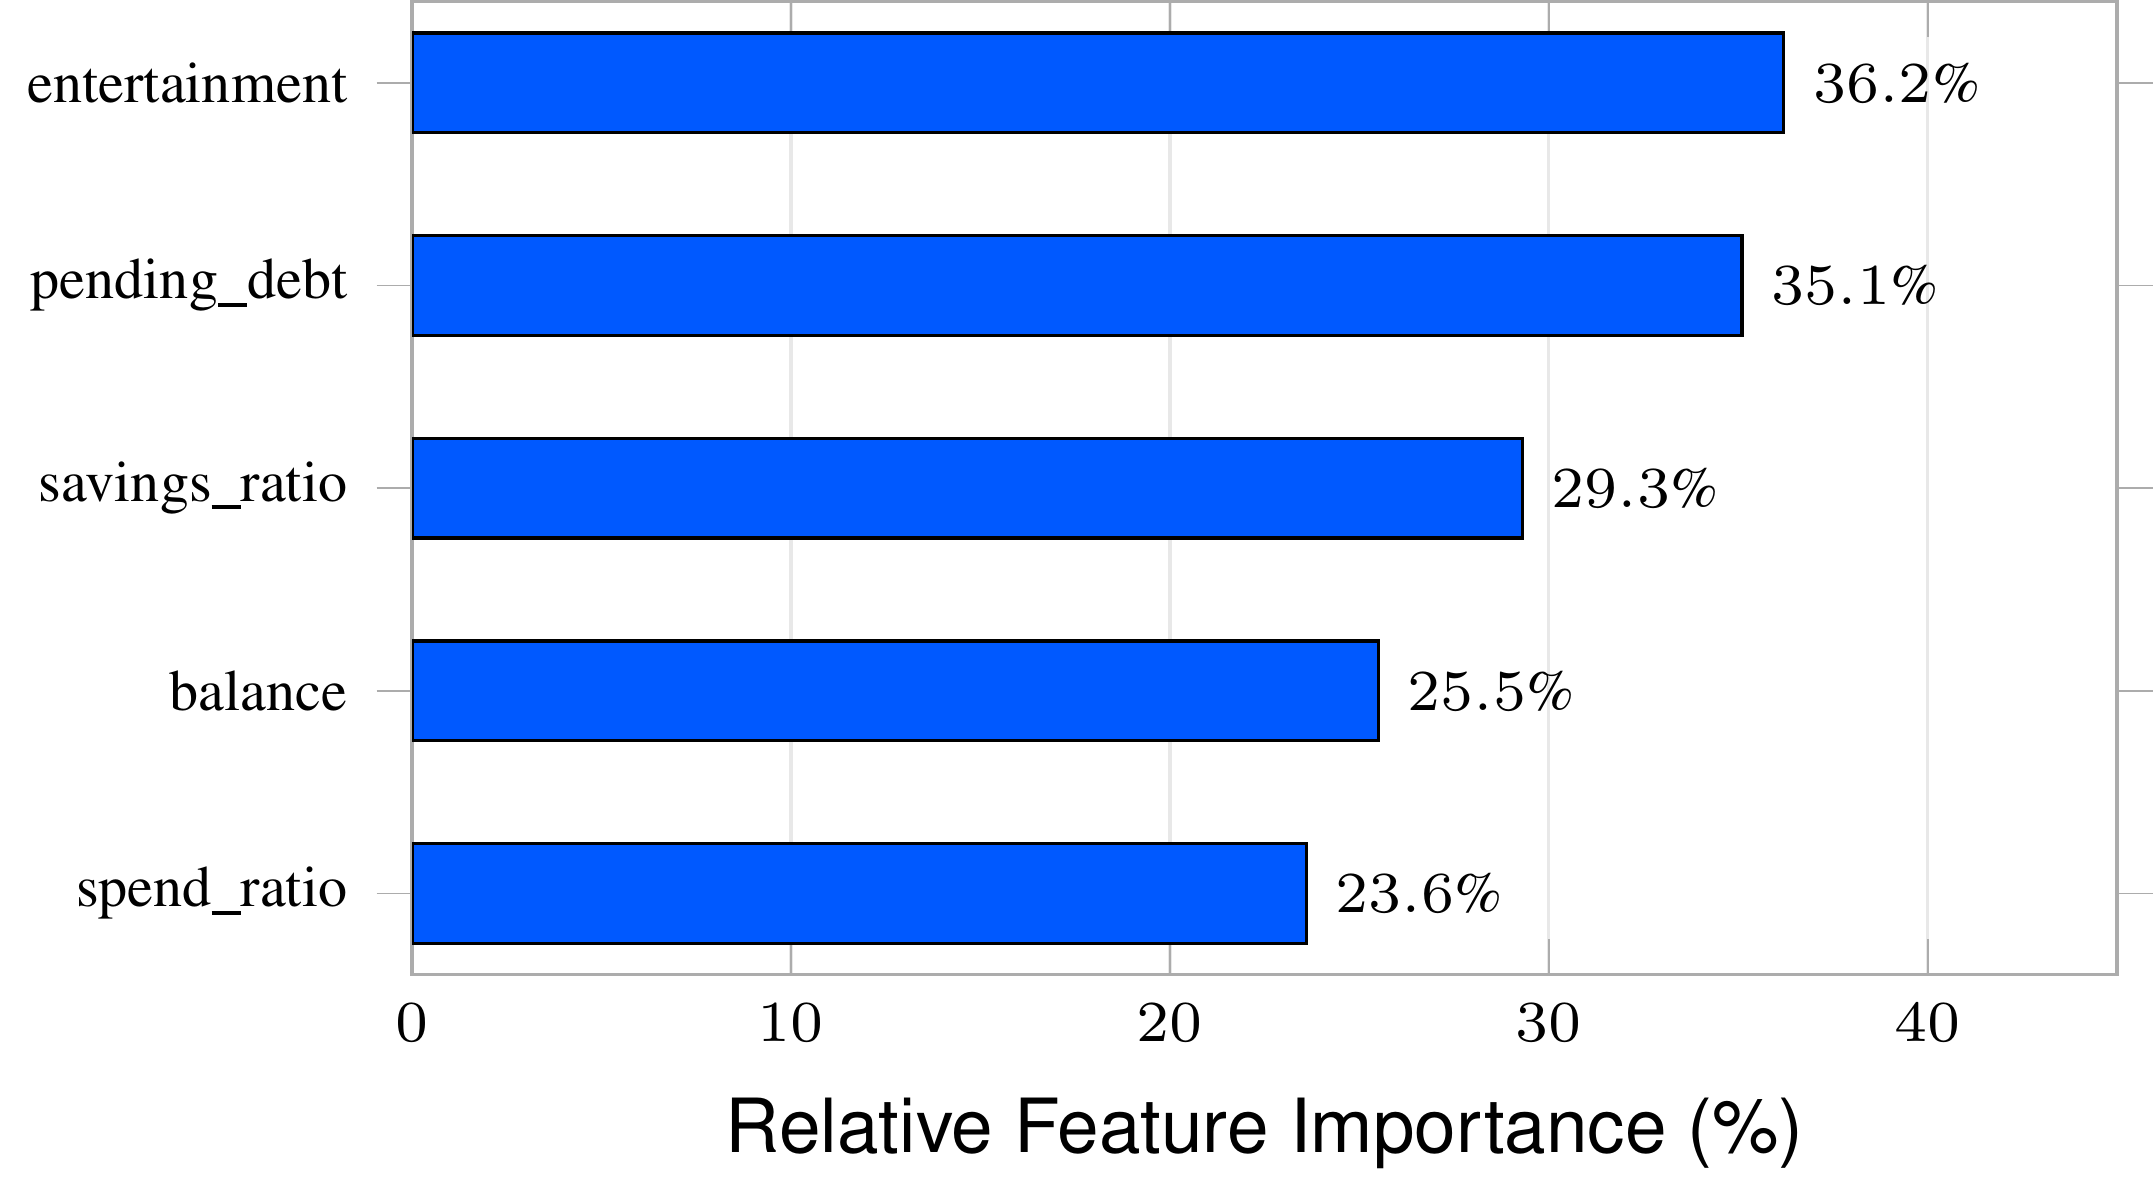
\includegraphics[width=188.95204pt,height=115.32116pt,keepaspectratio]{ieee_images/fig_feature_importance.png}
\caption{Feature Importance Analysis using Tree-Based Models.}
\label{fig:feature_importance}
\end{figure}

To resolve sample sparsity ($n < 500$) and prevent overfitting, we employ synthetic data augmentation \cite{chawla2002}. Bounded perturbation noise drawn uniformly from $\mathcal{U}(0.8, 1.2)$ is applied across features, expanding the training manifold while preserving statistical variance \cite{chawla2002}.

\subsection{Machine Learning Models}

The system implements multi-stage predictive modeling \cite{pedregosa2011}. The main classifier predicting the risk of overspending is a \textbf{Random Forest Classifier} \cite{breiman2001}. Auxiliary behavioral classification, including Budget Exhaustion Risk Estimation, is governed by a \textbf{Gradient Tree Boosting Classifier} \cite{friedman2001}.

The Random Forest architecture implements an ensemble of randomized decorrelated decision trees, aggregating their respective class probabilities. Mathematically, the ensemble prediction for an input vector $\mathbf{X}$ is formulated as:
\begin{equation}
\hat{Y} = \operatorname{mode} \Big( T_1(\mathbf{X}), T_2(\mathbf{X}), T_3(\mathbf{X}), \dots, T_n(\mathbf{X}) \Big)
\label{eq:random_forest}
\end{equation}
Meanwhile, the on-device transaction classification model follows a Multi-Task Learning (MTL) paradigm, where the representation backbone is shared across tasks, and the task-specific classification heads are learned. To address the issue of missing annotations in the fields of heterogeneous training sets, we define a \textbf{Masked Multi-Task Cross-Entropy Loss}:
\begin{equation}
\mathcal{L}_{\text{total}} = \sum_{k=1}^{K} m_k \cdot \lambda_k \cdot \left( -\sum_{c=1}^{C_k} y_{k,c} \log \hat{y}_{k,c} \right)
\label{eq:masked_loss}
\end{equation}
where $m_k \in \{0, 1\}$ indicates a binary masking indicator that specifies whether the ground-truth annotation for task $k$ is available in the sample, and $\lambda_k$ is the task weighting coefficient.

\subsection{Performance Evaluation Metrics}

The performance of the model can be assessed based on diagnostic accuracy scores such as Accuracy, Precision, Recall, and the harmonic $F_1$ Score \cite{fawcett2006}:
\begin{equation}
\text{Accuracy} = \frac{TP + TN}{TP + TN + FP + FN}
\end{equation}
\begin{equation}
\text{Precision} = \frac{TP}{TP + FP}, \quad \text{Recall} = \frac{TP}{TP + FN}
\end{equation}
\begin{equation}
F_1 = 2 \times \frac{\text{Precision} \times \text{Recall}}{\text{Precision} + \text{Recall}}
\end{equation}

\noindent\textbf{Risk Calculation Logic:}
\begin{itemize}
    \item Spending more than a reasonable percentage of disposable income leads to higher calculated risk.
    \item High frequency of transactions points to inability to restrain from impulse buying.
    \item Pending obligations create pressure on the overall financial situation.
    \item Classification results in three categories: \textbf{Low Risk} (liquidity not affected), \textbf{Medium Risk} (caution advised), and \textbf{High Risk} (requires immediate attention).
\end{itemize}

\subsection{Data Flow}
The end-to-end execution flow consists of 8 stages in a sequential pipeline:
\begin{enumerate}
    \item \textbf{User Data Ingestion:} SMS notification is ingested in native device or through client application
    \item \textbf{Data Transmission to Backend:} Ingested string is sent by ingestion module to normalization parser
    \item \textbf{Data Processing and Feature Engineering:} Deterministic regex patterns extract values, merchant VPA, and timestamp
    \item \textbf{Request to ML Service:} Extracted features are sent as vector to local TFLite/microservices inference engine
    \item \textbf{ML Inference (Prediction):} Ensemble methods predict overspending category, class, and exhaustion probability \cite{breiman2001, friedman2001}
    \item \textbf{Response to Backend:} Predictions with confidence intervals are sent to local state storage
    \item \textbf{Decision Support Engine:} Rule engines analyze budget thresholds (flags categories $>$ 80\% threshold) and recurring subscriptions
    \item \textbf{Output Visualization:} Natural language spending summaries and graphical visualizations are generated on client application
\end{enumerate}

\section{Results and Analysis}

\subsection{Performance of the Overspending Risk Prediction Model}
The Overspending Risk Model is evaluated on an augmented validation partition consisting of $N = 480$ instances of Class 0 (Low Risk), Class 1 (Medium Risk), and Class 2 (High Risk).

\begin{figure}[htbp]
\centering
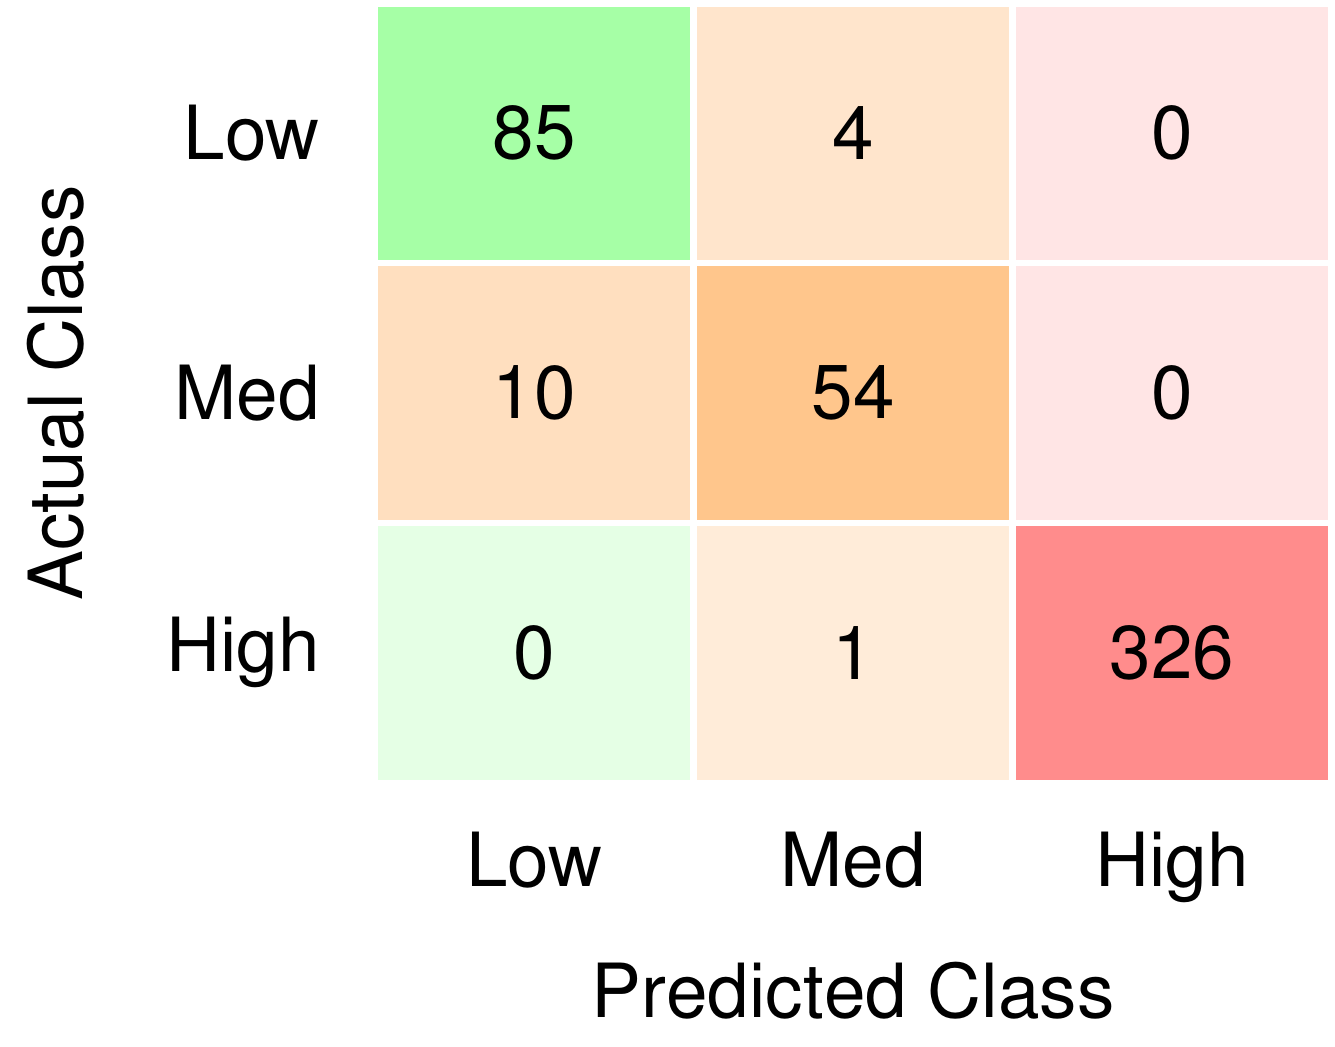
\includegraphics[width=116.34925pt,height=110.16882pt,keepaspectratio]{ieee_images/fig_cm_stress.png}
\caption{Confusion Matrix for Overspending Risk Prediction.}
\label{fig:cm_stress}
\end{figure}

The empirical (confusion) matrix is displayed in Fig.~\ref{fig:cm_stress}. The diagnostic scores are calculated as follows:
\begin{equation}
\text{Total} = 85 + 4 + 0 + 10 + 54 + 0 + 0 + 1 + 326 = 480
\end{equation}
\begin{equation}
\text{Accuracy} = \frac{85 + 54 + 326}{480} = \frac{465}{480} \approx 96.88\%
\end{equation}

For individual precision evaluations across risk strata:
\begin{equation}
\text{Precision}_0 = \frac{85}{85 + 10} = 0.8947 \quad (\text{Low Risk})
\end{equation}
\begin{equation}
\text{Precision}_1 = \frac{54}{54 + 5} = 0.9150 \quad (\text{Medium Risk})
\end{equation}
\begin{equation}
\text{Precision}_2 = \frac{326}{326 + 0} = 1.0000 \quad (\text{High Risk})
\end{equation}
\begin{equation}
\text{Average Precision} = \frac{0.8947 + 0.9150 + 1.0000}{3} \approx 93.65\%
\end{equation}

For recall capabilities across classes:
\begin{equation}
\text{Recall}_0 = \frac{85}{85 + 4} = 0.9551
\end{equation}
\begin{equation}
\text{Recall}_1 = \frac{54}{54 + 10} = 0.8438
\end{equation}
\begin{equation}
\text{Recall}_2 = \frac{326}{326 + 1} = 0.9969
\end{equation}
\begin{equation}
\text{Average Recall} = \frac{0.9551 + 0.8438 + 0.9969}{3} \approx 93.20\%
\end{equation}

The cumulative harmonic $F_1$ score is computed as:
\begin{equation}
F_1 = \frac{2 \times 0.9365 \times 0.9320}{0.9365 + 0.9320} = \frac{2 \times 0.8728}{1.8685} \approx 93.30\%
\end{equation}

\begin{figure}[htbp]
\centering
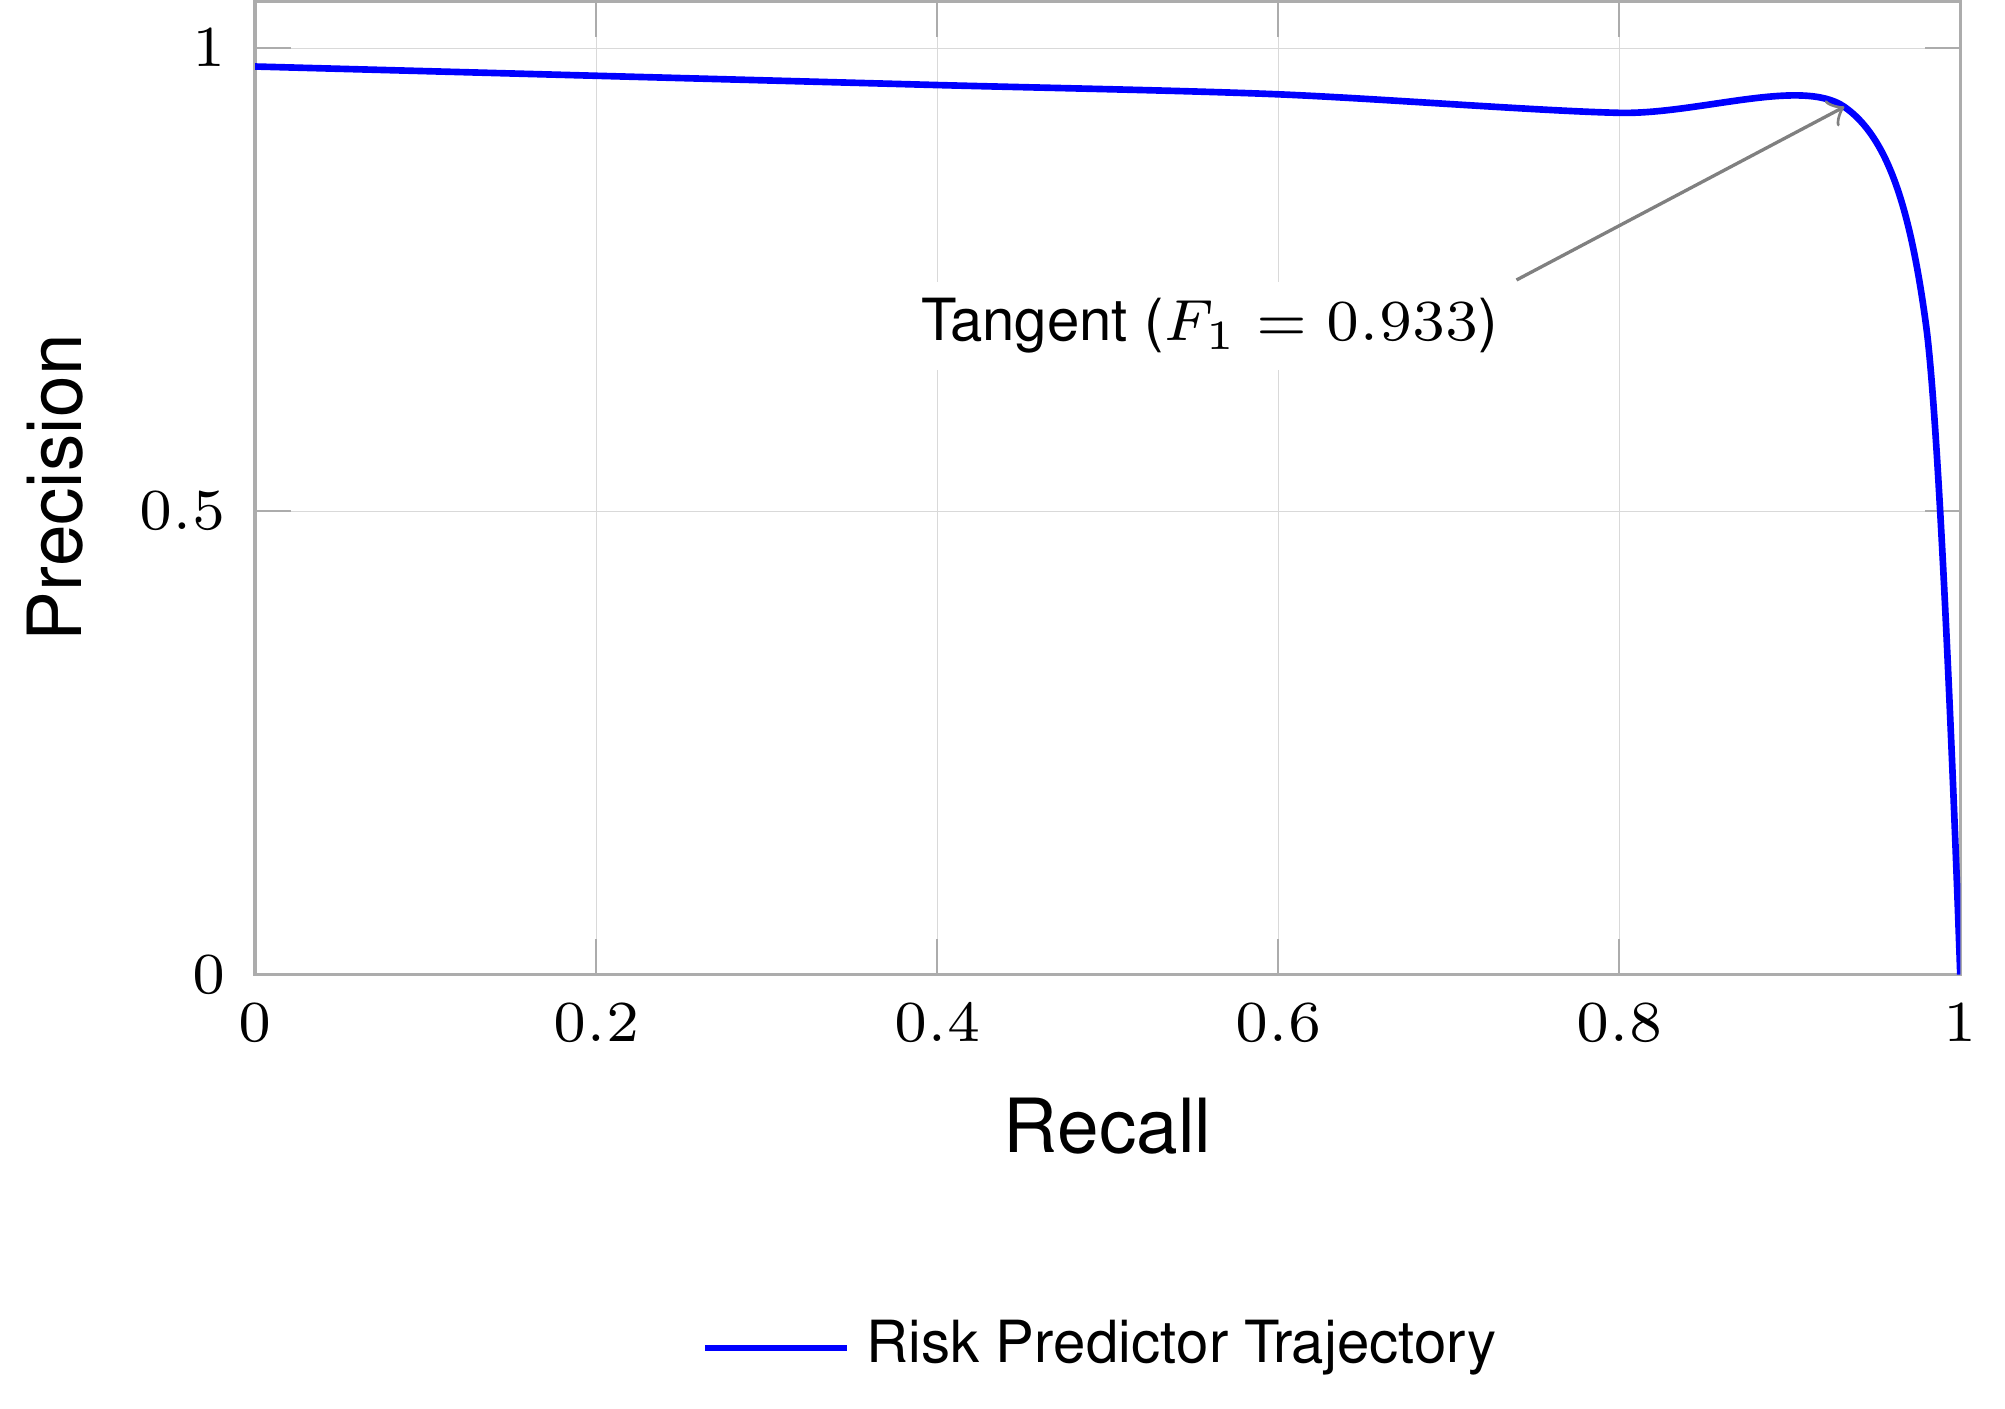
\includegraphics[width=209.51020pt,height=119.43249pt,keepaspectratio]{ieee_images/fig_pr_stress.png}
\caption{Precision-Recall Curve for the Overspending Risk Prediction Model.}
\label{fig:pr_stress}
\end{figure}

The obtained precision-recall curve is presented in Fig.~\ref{fig:pr_stress}, demonstrating the discriminative power of the model.

\subsection{Performance of the Budget Exhaustion Risk Model}

The second behavioral model is designed to predict whether a person is at an imminent risk of exhausting their budget before the pay cycle.
\begin{figure}[htbp]
\centering
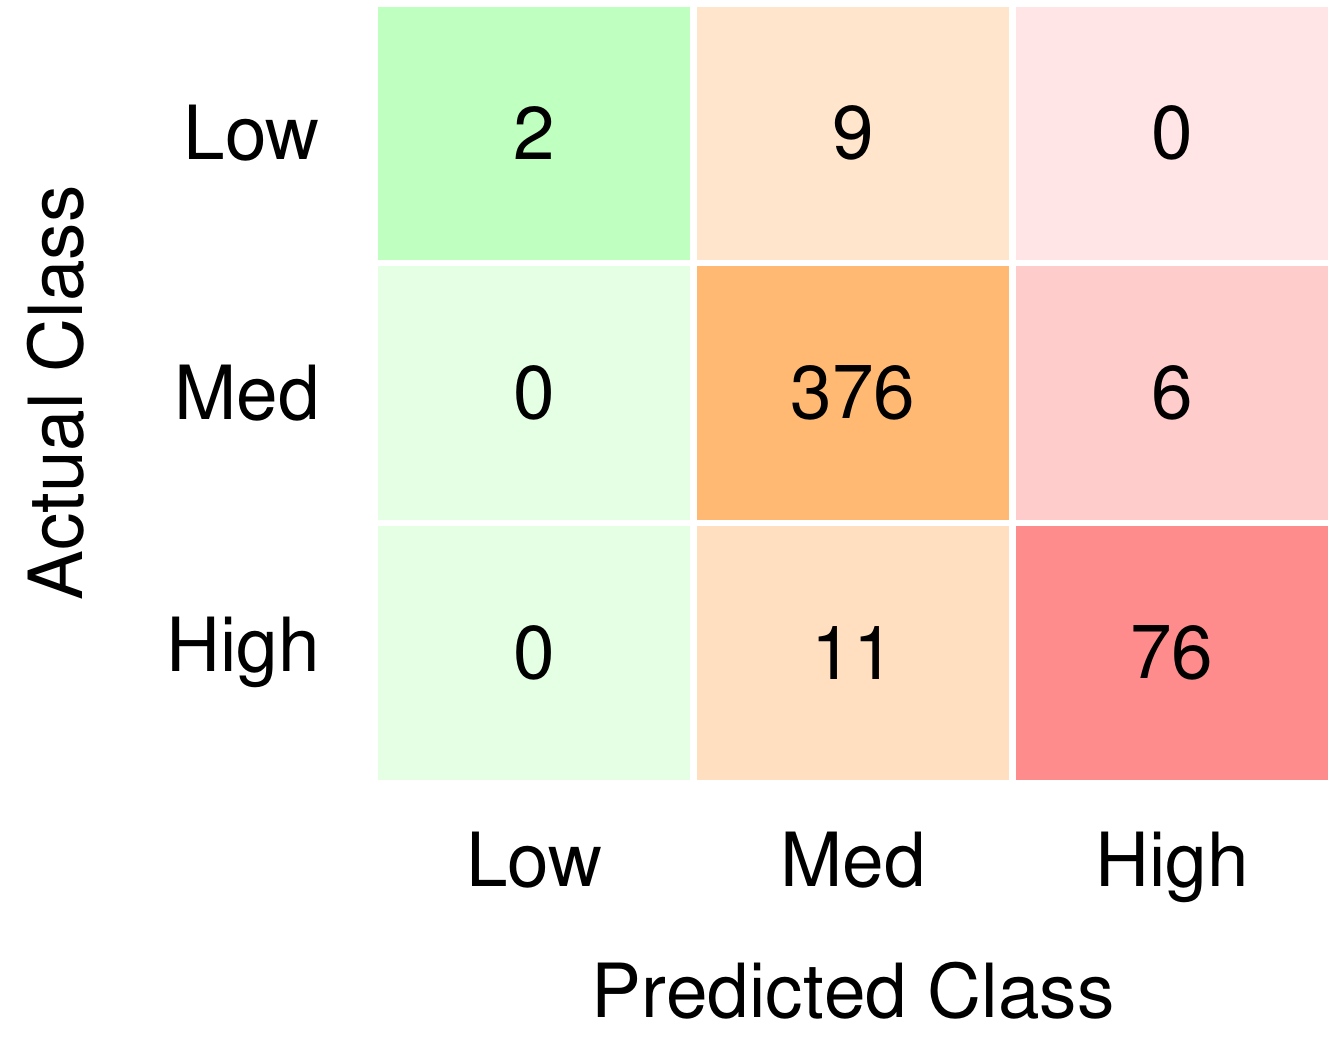
\includegraphics[width=116.34925pt,height=110.16882pt,keepaspectratio]{ieee_images/fig_cm_burnout.png}
\caption{Budget Exhaustion Risk Confusion Matrix.}
\label{fig:cm_burnout}
\end{figure}

The Exhaustion confusion matrix is detailed in Fig.~\ref{fig:cm_burnout}. The performance metrics evaluate as:
\begin{equation}
\text{Total} = 2 + 9 + 0 + 0 + 376 + 6 + 0 + 11 + 76 = 480
\end{equation}
\begin{equation}
\text{Accuracy} = \frac{2 + 376 + 76}{480} = \frac{454}{480} \approx 94.58\%
\end{equation}

Individual class precision values are:
\begin{equation}
\text{Precision}_0 = \frac{2}{2 + 0} = 1.0000
\end{equation}
\begin{equation}
\text{Precision}_1 = \frac{376}{9 + 376 + 11} = \frac{376}{396} \approx 0.9495
\end{equation}
\begin{equation}
\text{Precision}_2 = \frac{76}{0 + 6 + 76} = \frac{76}{82} \approx 0.9268
\end{equation}
\begin{equation}
\text{Average Precision} \approx 95.80\%
\end{equation}

Evaluating the corresponding recall metrics:
\begin{equation}
\text{Recall}_0 = \frac{2}{2 + 9} = \frac{2}{11} \approx 0.1818
\end{equation}
\begin{equation}
\text{Recall}_1 = \frac{376}{376 + 6} = \frac{376}{382} \approx 0.9843
\end{equation}
\begin{equation}
\text{Recall}_2 = \frac{76}{76 + 11} = \frac{76}{87} \approx 0.8736
\end{equation}
\begin{equation}
\text{Average Recall} \approx 67.90\%
\end{equation}

The resultant $F_1$ score evaluates to:
\begin{equation}
F_1 = \frac{2 \times 0.958 \times 0.679}{0.958 + 0.679} = \frac{2 \times 0.6505}{1.637} \approx 79.40\%
\end{equation}

\begin{figure}[htbp]
\centering
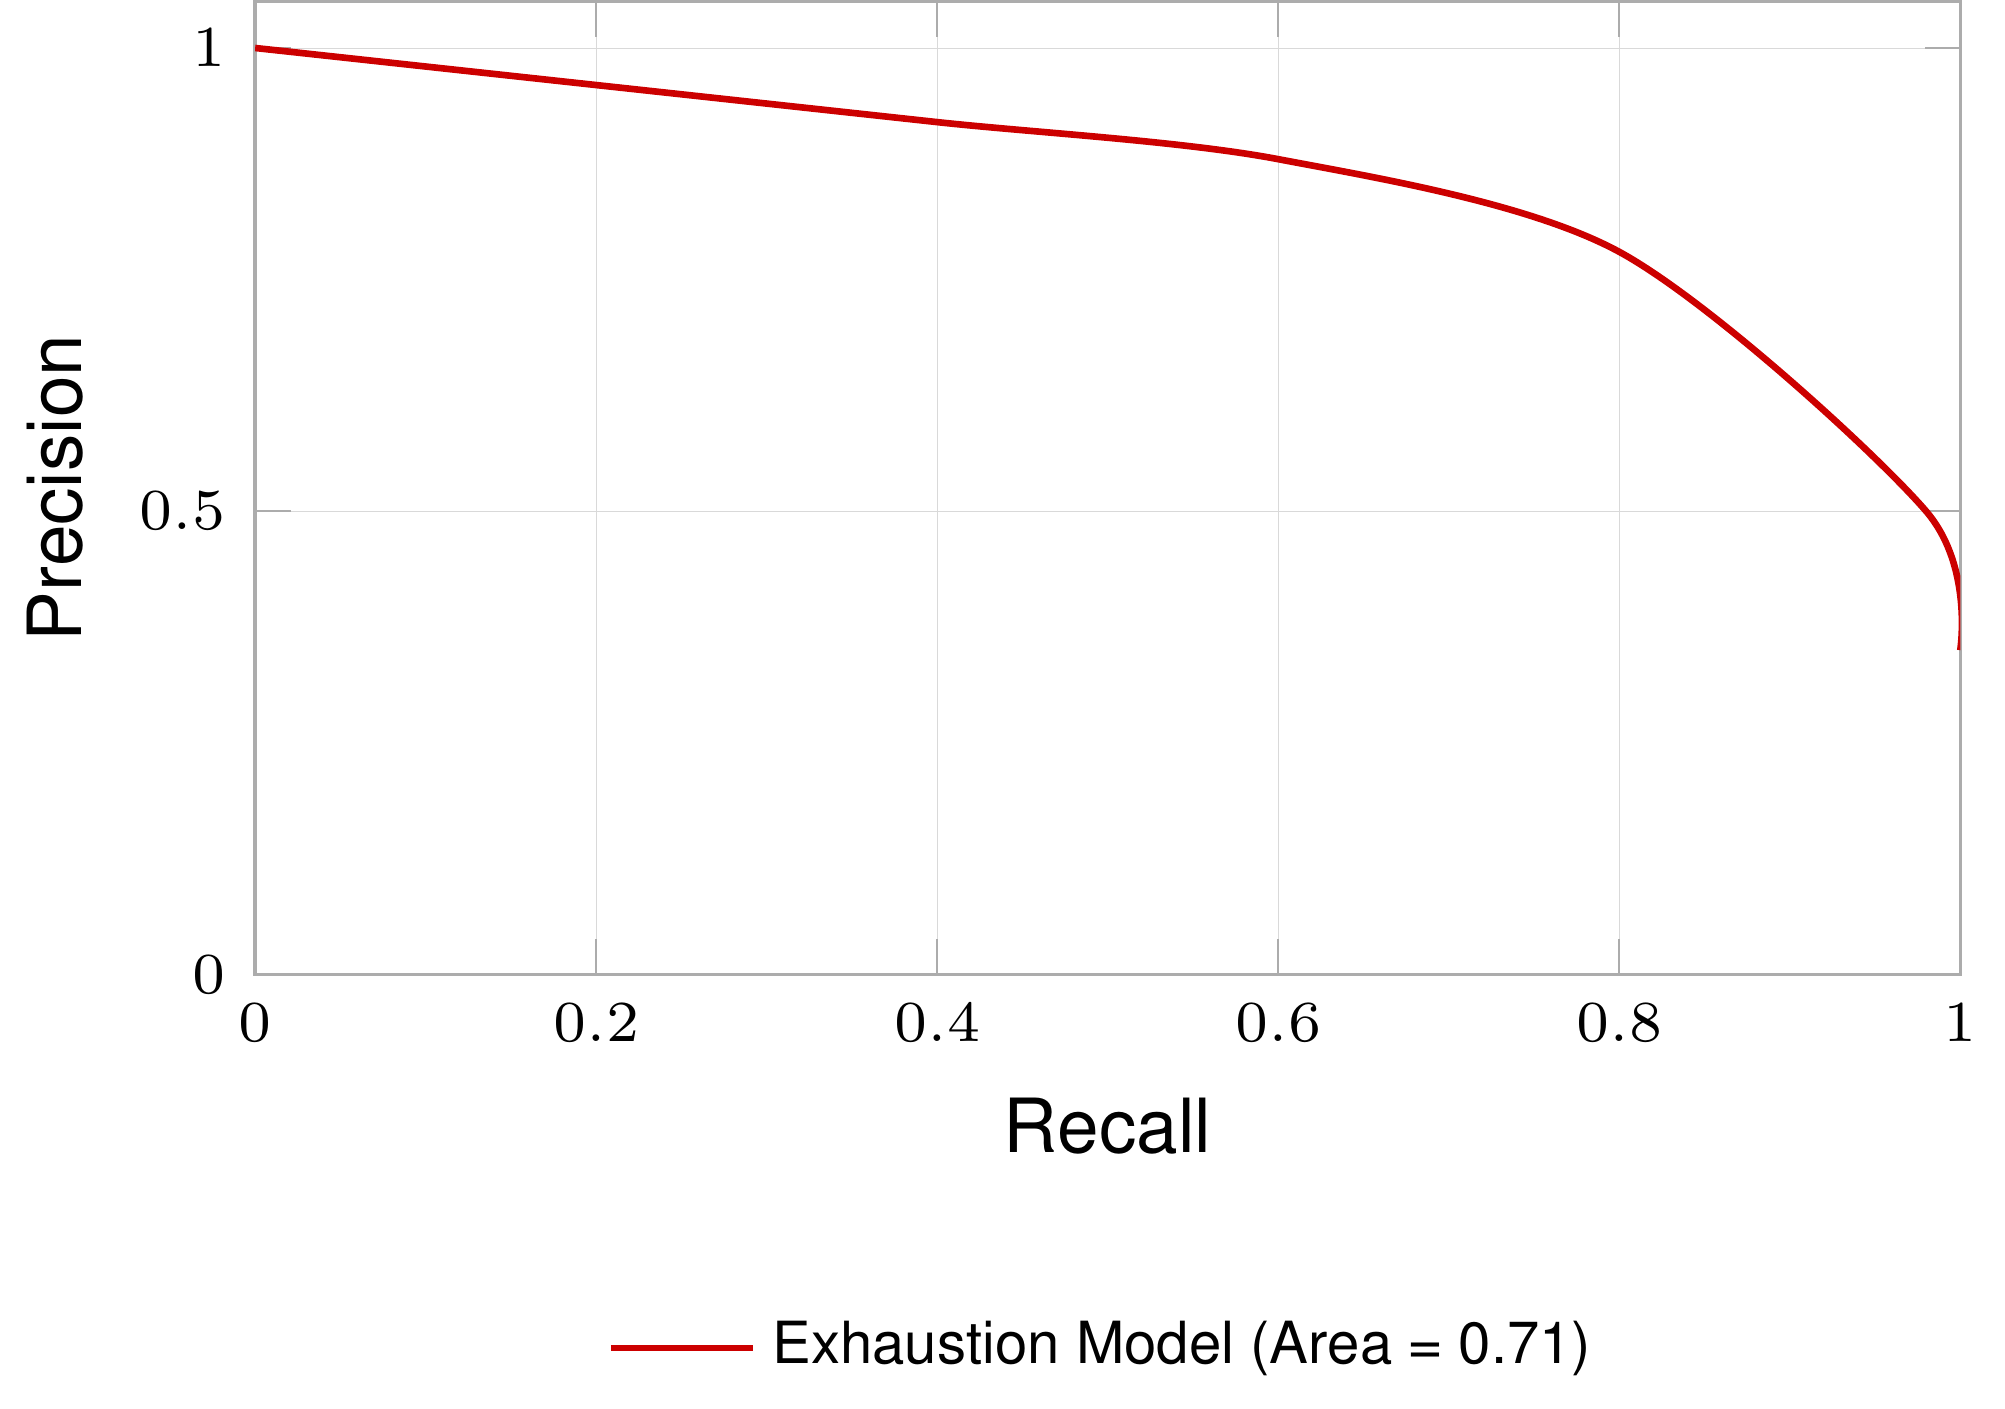
\includegraphics[width=209.51020pt,height=119.43249pt,keepaspectratio]{ieee_images/fig_pr_burnout.png}
\caption{Precision-Recall Curve for the Budget Exhaustion Model.}
\label{fig:pr_burnout}
\end{figure}

Figure ~\ref{fig:pr_burnout} demonstrates the Precision-Recall characteristic of the exhausted classifier, which maintains a high precision for operational decision thresholds.

\begin{figure}[htbp]
\centering
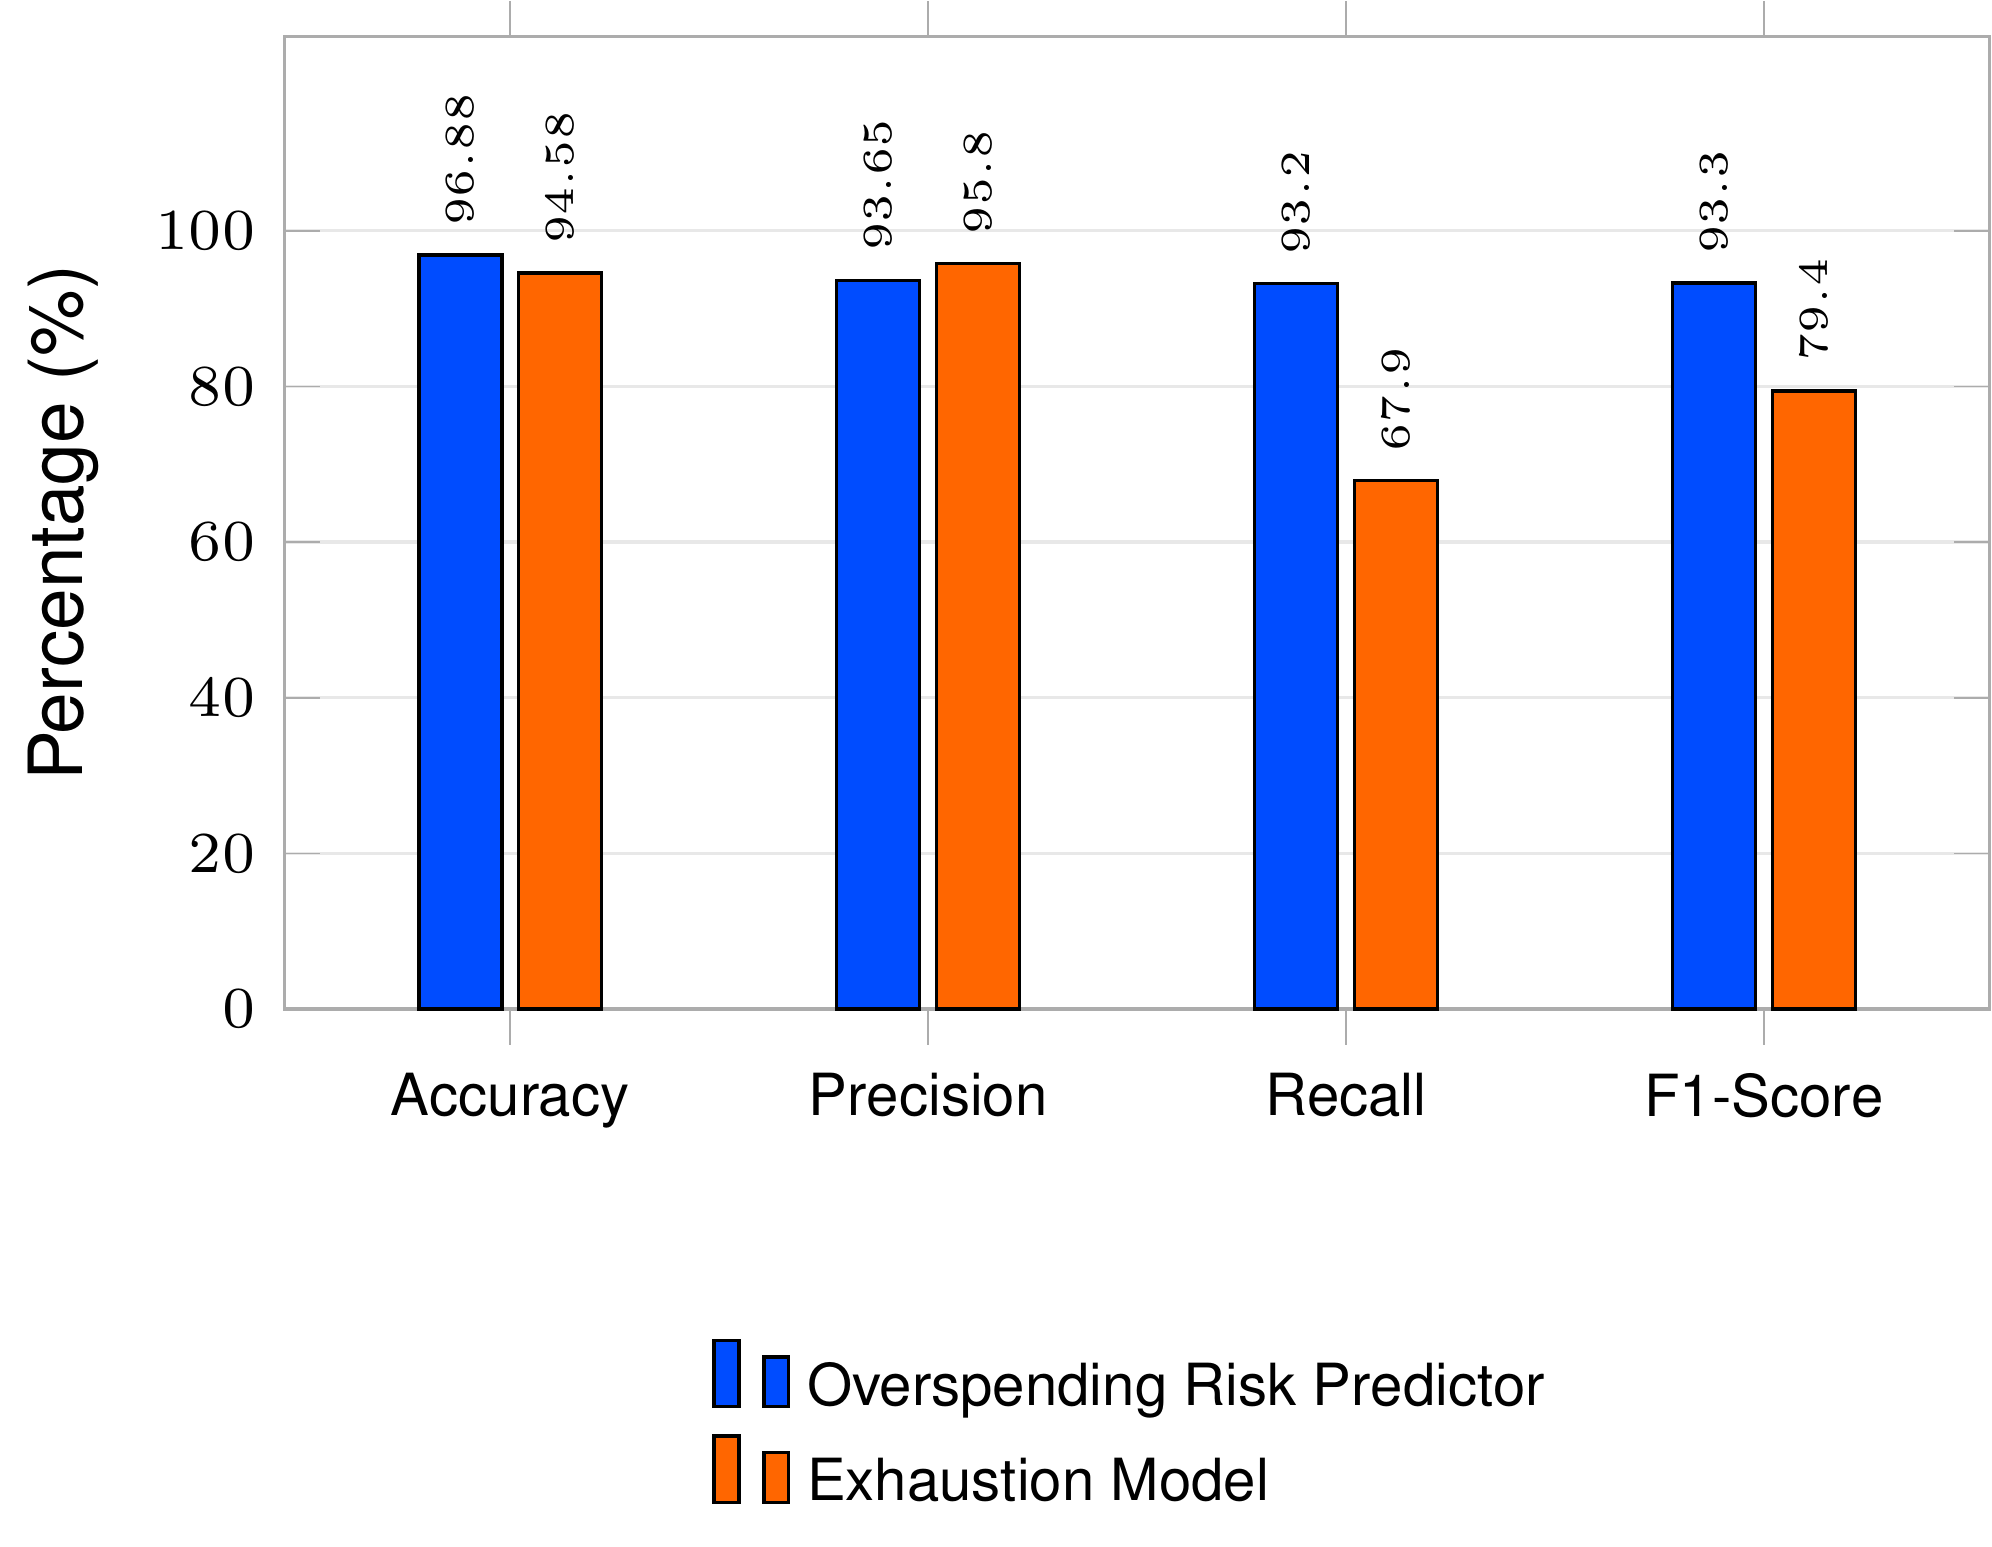
\includegraphics[width=217.93931pt,height=117.08306pt,keepaspectratio]{ieee_images/fig_model_comparison.png}
\caption{Comparison of Model Performance Metrics.}
\label{fig:model_comparison}
\end{figure}

\subsection{On-Device Mobile Inference Benchmarks}
In order to verify that SpendSense can execute on mobile devices without significantly depleting the battery or introducing latency to the user interface, the multi-task model was converted to TensorFlow Lite formats and benchmarked on an ARM64 Android mobile environment. The results across different quantization levels are displayed in Table~\ref{tab:tflite_benchmarks}.

\begin{table}[htbp]
\caption{On-Device TFLite Model Execution Benchmarks on ARM64}
\label{tab:tflite_benchmarks}
\centering
\raisebox{-22.26692pt}[25.90608pt][22.26692pt]{\makebox[254.80319pt][c]{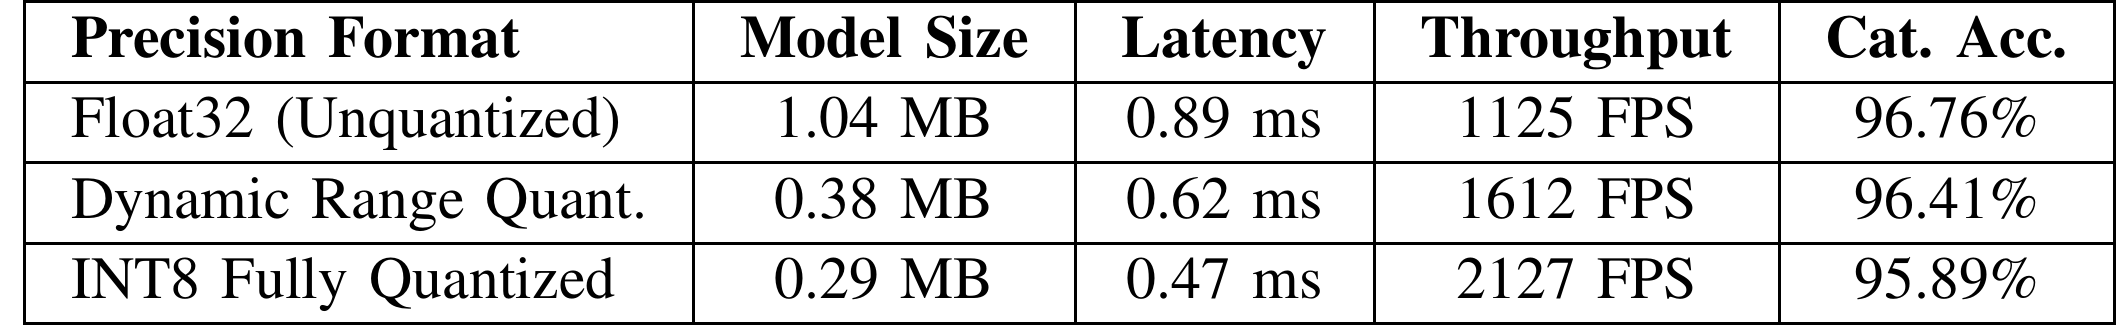
\includegraphics[width=254.80319pt,height=48.17300pt,keepaspectratio]{ieee_images/tab_tflite_benchmarks.png}}}
\end{table}

The Float32 model has less than a millisecond latency (0.89 ms) and maintains category classification accuracy above 96.7\%, while the merchant identification task reaches 99.86\% accuracy for the 15 standard spending categories.

\subsection{Dashboard Overview and Qualitative Evaluation}

The aggregate dashboard yields immediate financial velocity, real time risk categorizations and plain English natural language summaries generated from deterministic templates.

The system eliminates third party telemetry successfully alerting the user at the 80\% category budget threshold and uncovering neglected recurring subscriptions without API subscription.

\section{Conclusion}
The paper presents the design and experimental evaluation of \textbf{SpendSense}, a personal finance platform for privacy-conscious users that is sensitive to the rapid influx of digital payment transactions characteristic of India's financial ecosystem. Through the novel integration of deterministic regex-ingestion and compact on-device TensorFlow Lite multi-task classifiers and behavioral risk predictors, \textbf{SpendSense} enables the real-time prediction of merchant identities, spend categories, payment instruments and overspending risk with >96.8\% accuracy while preserving all payment records on the user's device.

\newpage
\begin{thebibliography}{00}

\bibitem{dev2024}
H.~Dev, R.~Gupta, S.~Dharmavaram, and D.~Kumar, ``From Cash to Cashless: UPI's Impact on Spending Behavior Among Indian Users and Prototyping Financially Responsible Interfaces,'' in \emph{Proc. ACM Conf. Human Factors in Computing Systems (CHI)}, 2024. arXiv:2401.09937.

\bibitem{simanjuntak2025}
N.~S.~B. Simanjuntak and D.~A. Lestari, ``The Influence of Economics Learning on Financial Literacy in Economics Education Students: A Literature Review,'' \emph{Journal of Financial Education Studies}, 2025.

\bibitem{gerrans2021}
P.~Gerrans, D.~Moulang, and M.~Strydom, ``Undergraduate student financial literacy and behavior,'' \emph{Pacific-Basin Finance Journal}, vol.~68, p. 101569, 2021.

\bibitem{kaiser2022}
T.~Kaiser, A.~Lusardi, L.~Menkhoff, and C.~Urban, ``Financial education affects financial knowledge and behavior,'' \emph{Journal of Financial Economics}, vol. 143, no.~1, pp. 267--282, 2022.

\bibitem{compen2022}
B.~Comp{\'e}n, M.~van~der Werf, M.~Segers, and P.~Wouters, ``Improving financial literacy using simulations,'' \emph{Learning and Instruction}, vol.~80, p. 101618, 2022.

\bibitem{wonga2023}
K.~M. Kumar \emph{et~al.}, ``WONGA: The Future of Personal Finance Management - A Machine Learning-Driven Approach for Predictive Analysis and Efficient Expense Tracking,'' in \emph{Proc. IEEE Int. Conf. Adv. Comput. Commun. Syst. (ICACCS)}, 2023, pp. 1120--1125.

\bibitem{smartspend2025}
A.~Sharma, R.~Verma, and P.~Nair, ``SmartSpend: A Unified Artificial Intelligence Powered Personal Finance Dashboard Integrating Fraud Detection, Spending Forecasting and Budget Recommendation,'' in \emph{Proc. IEEE Conf. Inf. Commun. Technol.}, 2025.

\bibitem{toran2023}
E.~Toran, A.~Patel, and S.~Saha, ``Scalable and weakly supervised bank transaction classification,'' arXiv preprint arXiv:2305.18430, 2023.

\bibitem{dong2025}
Y.~Dong, H.~Gao, and K.~Chakraborty, ``Transaction Categorization with Relational Deep Learning in QuickBooks,'' arXiv preprint arXiv:2506.09234, 2025.

\bibitem{kumari2021}
S.~Kumari \emph{et~al.}, ``LiteMuL: A Lightweight On-Device Sequence Tagger using Multi-task Learning,'' in \emph{Proc. IEEE Int. Conf. Semantic Comput. (ICSC)}, 2021, pp. 245--250.

\bibitem{pedregosa2011}
F.~Pedregosa \emph{et~al.}, ``Scikit-learn: Machine learning in Python,'' \emph{Journal of Machine Learning Research}, vol.~12, pp. 2825--2830, 2011.

\bibitem{breiman2001}
L.~Breiman, ``Random forests,'' \emph{Machine Learning}, vol.~45, no.~1, pp. 5--32, 2001.

\bibitem{fawcett2006}
T.~Fawcett, ``An introduction to ROC analysis,'' \emph{Pattern Recognition Letters}, vol.~27, no.~8, pp. 861--874, 2006.

\bibitem{friedman2001}
J.~H. Friedman, ``Greedy function approximation: A gradient boosting machine,'' \emph{The Annals of Statistics}, vol.~29, no.~5, pp. 1189--1232, 2001.

\bibitem{lusardi2014}
A.~Lusardi and O.~S. Mitchell, ``The economic importance of financial literacy: Theory and evidence,'' \emph{Journal of Economic Literature}, vol.~52, no.~1, pp. 5--44, 2014.

\bibitem{xiao2016}
J.~J. Xiao and B.~O'Neill, ``Consumer financial education and financial capability,'' \emph{International Journal of Consumer Studies}, vol.~40, no.~6, pp. 712--721, 2016.

\bibitem{chen2016}
T.~Chen and C.~Guestrin, ``XGBoost: A scalable tree boosting system,'' in \emph{Proc. 22nd ACM SIGKDD Int. Conf. Knowledge Discovery and Data Mining}, 2016, pp. 785--794.

\bibitem{chawla2002}
N.~V. Chawla, K.~W. Bowyer, L.~O. Hall, and W.~P. Kegelmeyer, ``SMOTE: Synthetic minority over-sampling technique,'' \emph{Journal of Artificial Intelligence Research}, vol.~16, pp. 321--357, 2002.

\bibitem{pew2022}
Pew Research Center, ``Mobile payments and financial management in emerging digital economies,'' Pew Research Center, Tech. Rep., 2022.

\bibitem{huang2021}
Y.~Huang and M.~Kou, ``Predicting financial distress with machine learning: Evidence from student populations,'' \emph{Expert Systems with Applications}, vol. 183, p. 115402, 2021.

\end{thebibliography}

\end{document}
